\section{Pre-requisites and compilation}
\label{devdocs}

The complete source code for the application is included on the DVD.
It is also available from the subversion repository at:

\texttt{http://svn.davidsansome.com/3yp}

\bigskip
\noindent Before compiling you should make sure you have the following libraries and tools installed:

\begin{enumerate}
	\item \textbf{CMake} (\texttt{http://www.cmake.org}).
	\item \textbf{Qt} (\texttt{http://www.trolltech.com}).
		Version 4.4 is \emph{required} as the modelfitter application uses the new QtConcurrent framework.
		At the time of writing Qt 4.4 was in release-candidate stage.
	\item \textbf{SVL} (\verb+http://www.cs.cmu.edu/~ajw/doc/svl.html+).
		I have created an Ubuntu package for SVL which is available from: \\
		\texttt{http://www.davidsansome.com/svl}.
	\item \textbf{ZLib} (\texttt{http://www.zlib.net/}).
	\item \textbf{FFTW} (\texttt{http://www.fftw.org/}).
	\item \textbf{GnuPlot} (\texttt{http://www.gnuplot.info/}).
		Optional - but the GnuPlot executable should be installed and in the \$PATH at runtime if you want to use the application's graph plotting features.
\end{enumerate}

The application should compile cleanly on Linux, Mac OS X and Windows.
Windows users are advised to use MinGW instead of Visual Studio.
To build the application you should issue the following commands:

\begin{lstlisting}[firstnumber=1,language=sh,frame=single,morekeywords={cmake,make}]
cd modelfitting/bin
cmake ..
make
./modelfitting
\end{lstlisting}

\section{Code structure}

The GUI part of the application is controlled by the MainWindow class.
This class is responsible for managing the menubars, toolbars, dock windows, and the four GLView objects that display the front, side, overhead and perspective views to the user.
The relationship between MainWindow and a few other important classes is shown in Figure \ref{MainClasses}.

Each frame in a video sequence is represented by an instance of the FrameInfo class.
Typically there will only be one full FrameInfo object instantiated at any one time during the lifecycle of the application, as it has quite a large memory footprint.
Frames are loaded by \emph{FrameModel::loadFrame} which returns a pointer to a new FrameInfo object (the caller is responsible for destroying this object later).
This function takes a boolean argument \emph{loadInfoOnly}.
If this is true then only the .info file associated with the frame will be loaded, otherwise both the info and the voxel data will be read into memory.

Whenever MainWindow loads a new frame, it will call \emph{setFrameInfo} on all four of the GLViews and the graph plotting classes to inform them of the change.

The model information is updated by a call to \emph{FrameInfo::update}.
This starts a number of background threads which perform the actual work of modelfitting, and returns immediately with a list of QFuture objects.
A QFuture is part of the new QtConcurrent framework and holds the result of an asynchronous operation.
MainWindow will open a modal dialog, MapReduceProgress, that monitors the progress of these QFuture objects and allows the user to cancel them.

\begin{landscape}
	\begin{figure}[p]
		\centering
		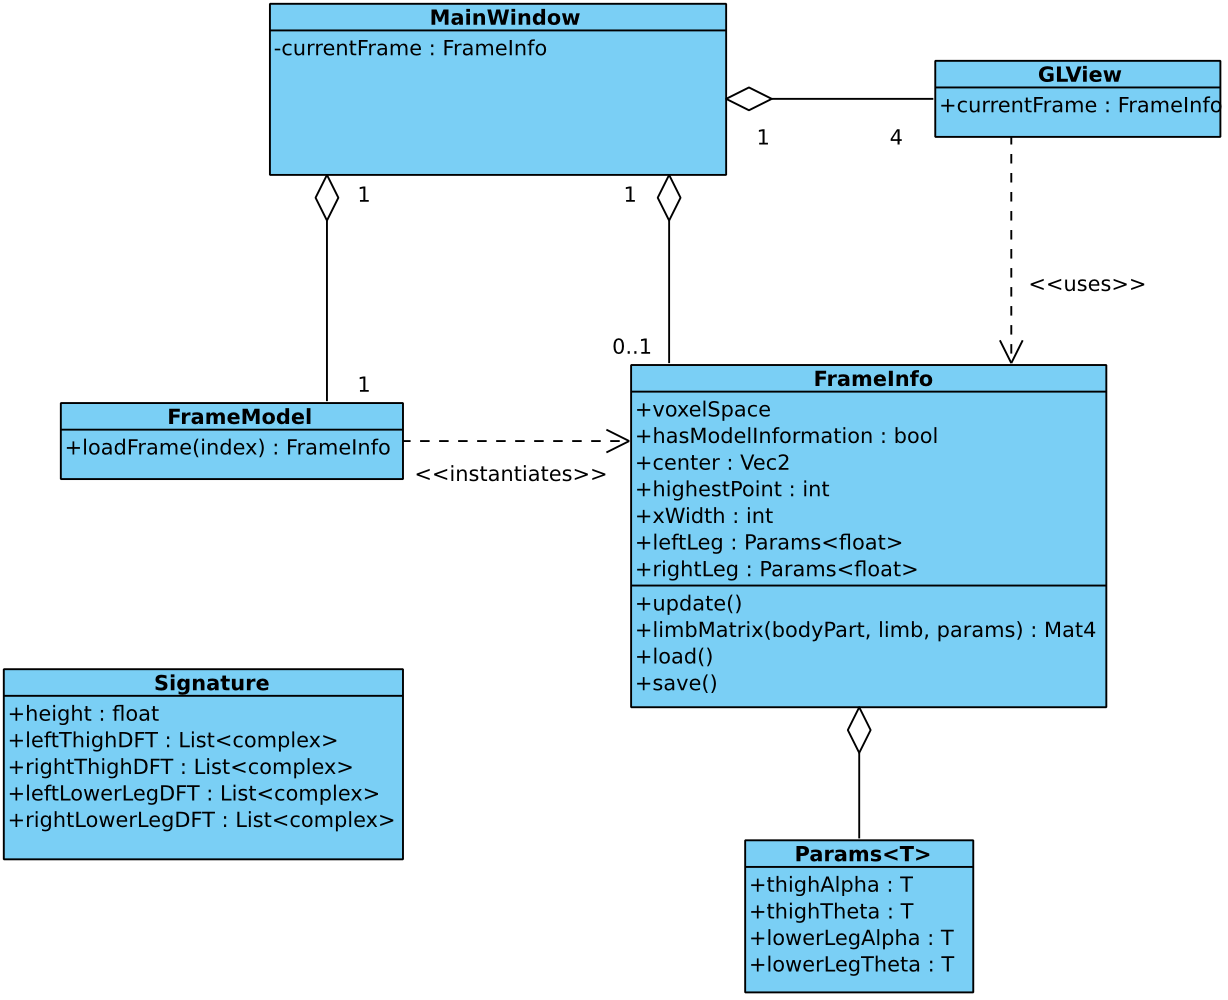
\includegraphics[width=\textwidth]{uml/mainwindow.png}
		\caption{The main classes in the application.}
		\label{MainClasses}
	\end{figure}
	
	\begin{figure}[p]
		\centering
		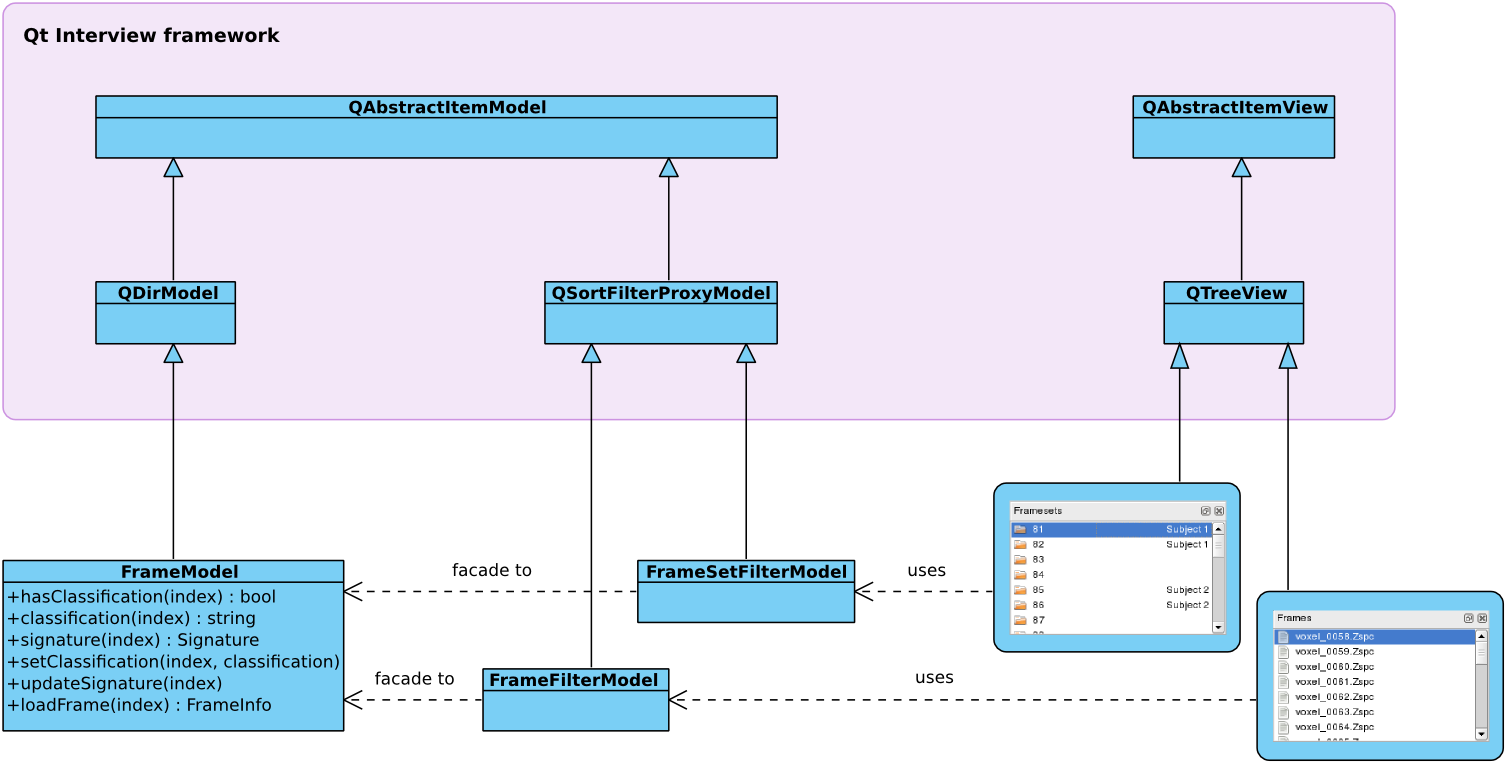
\includegraphics[width=20cm]{uml/interview.png}
		\caption{Model view architecture.}
		\label{ModelView}
	\end{figure}
\end{landscape}

The FrameModel class was only briefly mentioned before as being responsible for loading FrameInfo objects.
FrameModel is a subclass of QDirModel and manages access to lists of frames and framesets (directories of frames) on disk.
It can be used as the model for QAbstractItemView classes, such as the QTreeViews that appear in the left dock of MainWindow.
Each item in the model (frame or frameset) is indexed by a QModelIndex class, and all the functions in the FrameModel take such an index when operating on a frame or frameset.

Two filter models are provided (see Figure \ref{ModelView}) that filter out either framesets (directories) or frames (files that end in .Zspc).
These are not proper models themselves, but instead are facades to the real FrameModel.
As they both implement the QAbstractItemModel interface they can be provided directly to views.

This approach of managing access to frames through a single model is advantageous in several respects.
Firstly, it is good from a software engineering point of view - the MVC pattern is well used and generally accepted as being worthwhile.
Secondly, any views automatically get updated when a change is made to the model (eg. a frameset is classified by the user).

However the use of filters does add complexity when trying to use the model.
The Qt classes are implemented in such a way that an index into one of the filters can not immediately be used to index into the source model - it has to first be \emph{mapped} with \emph{QAbstractProxyModel::mapToSource}.
Thus, every class that wants to obtain a list of frames from a frameset, such as the Fft class, must hold onto its own FrameFilterModel instance and implement code similar to that in Listing \ref{IterateOverFrames}.

\begin{lstlisting}[firstnumber=1,language=c++,frame=single,caption={Code snippet to iterate over the frames in a frameset.},label={IterateOverFrames},float=[htb]]
FrameFilterModel* filter = new FrameFilterModel;
filter->setSourceModel(m_model);
filter->setRootIndex(frameSetIndex);
...
int count = filter->rowCount(filter->mapFromSource(frameSetIndex));

for (int i=0 ; i<count ; ++i)
{
	QModelIndex index(filter->mapToSource(filter->mapFromSource(frameSetIndex).child(i, 0)));
	// Do something with index
}
\end{lstlisting}

